\chapter{Results}
This chapter contains the results of both the mesh generation, which serves as input for the FEM calculation, and the results of the FEM calculations themselves

\section{Mesh generation}
As mentioned before the generation of the mesh is done using a separate program called Gmsh. In Gmsh a geometry is created which is then used to generate a mesh. This mesh can then be saved as a .msh file. Figure \ref{Gmsh}(a) shows the used geometry, and figure \ref{Gmsh}(b) shows the mesh resulting from this geometry. In this geometry the bottom left corner is fixed completely while the rest of the left hand side is only fixed in the x direction. A force is then placed on the right hand side. 

 \begin{figure}[H]
 	\begin{center}
    \subfigure[Geometry]{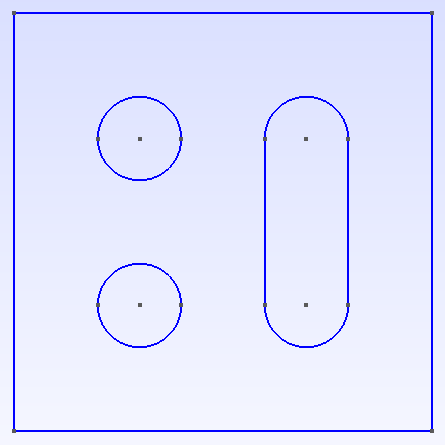
\includegraphics[width=0.45\textwidth]{IMG/Gmsh.png}}
    \subfigure[Mesh]{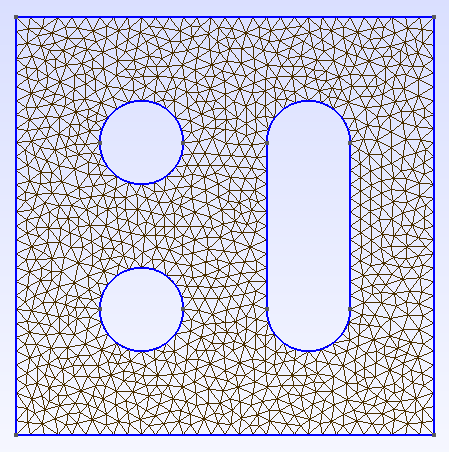
\includegraphics[width=0.45\textwidth]{IMG/Gmsh_msh.png}}
    \caption{Gmsh output}
    \label{Gmsh}
	\end{center}
\end{figure}
%
%\begin{figure}[H]
%    \begin{center}
%    \includegraphics[scale=0.5]{Illustrated}
%    \caption{Problem domain}
%    \label{FIG_problemdomain}
%    \end{center}
%\end{figure}

\section{FEM}
The resulting mesh is saved in a .msh file which is read by the FEM code. The code then does all the required calculations and the results are exported to paraview. The resulting images are shown below. Figure \ref{Disp} shows the displacement data. 

 \begin{figure}[H]
 	\begin{center}
    \subfigure[X displacement]{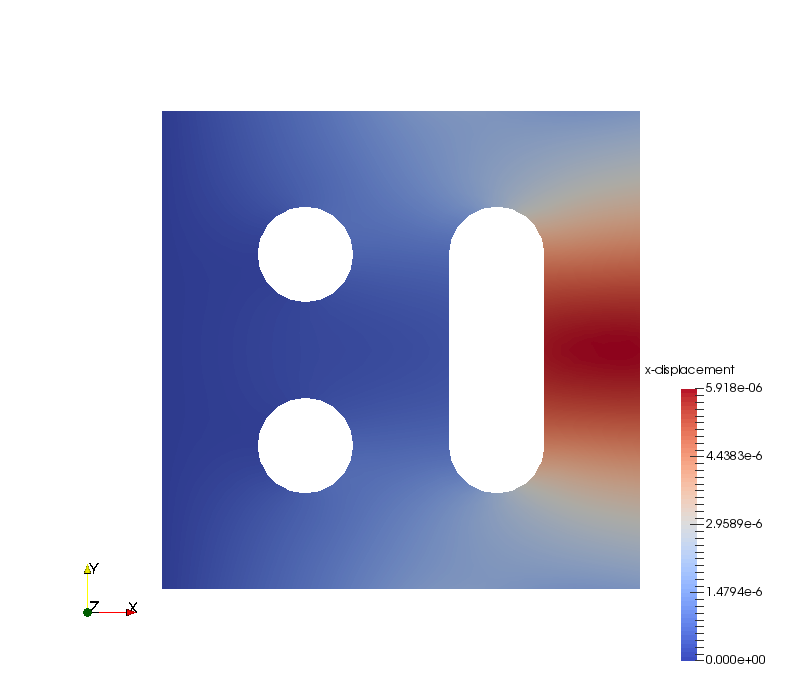
\includegraphics[width=0.49\textwidth]{IMG/smile_x_disp.png}}
    \subfigure[Y displacement]{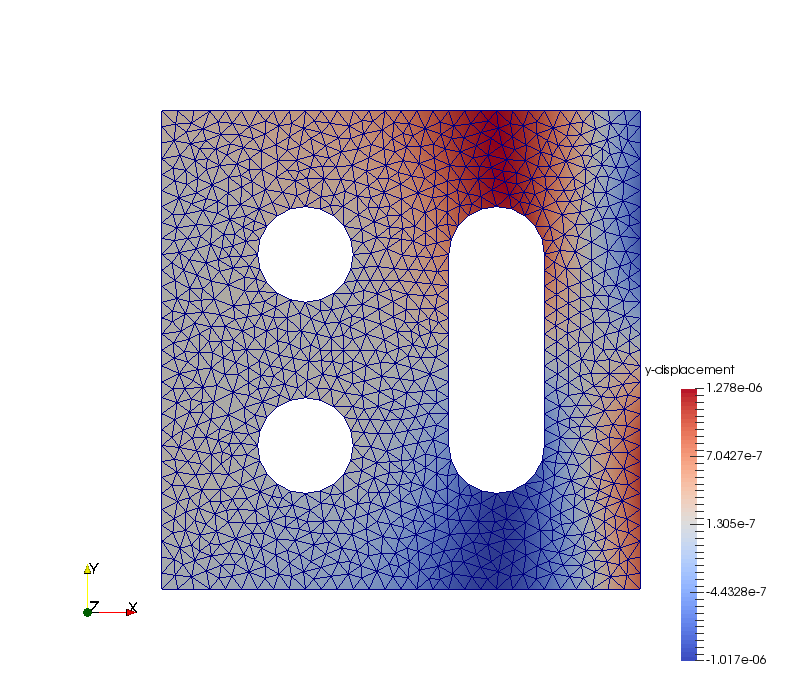
\includegraphics[width=0.49\textwidth]{IMG/smile_y_disp.png}}
    \caption{Displacement}
    \label{Disp}
	\end{center}
\end{figure}

And figure \ref{VonMises} shows the Von Mises stress.

\begin{figure}[H]
    \begin{center}
    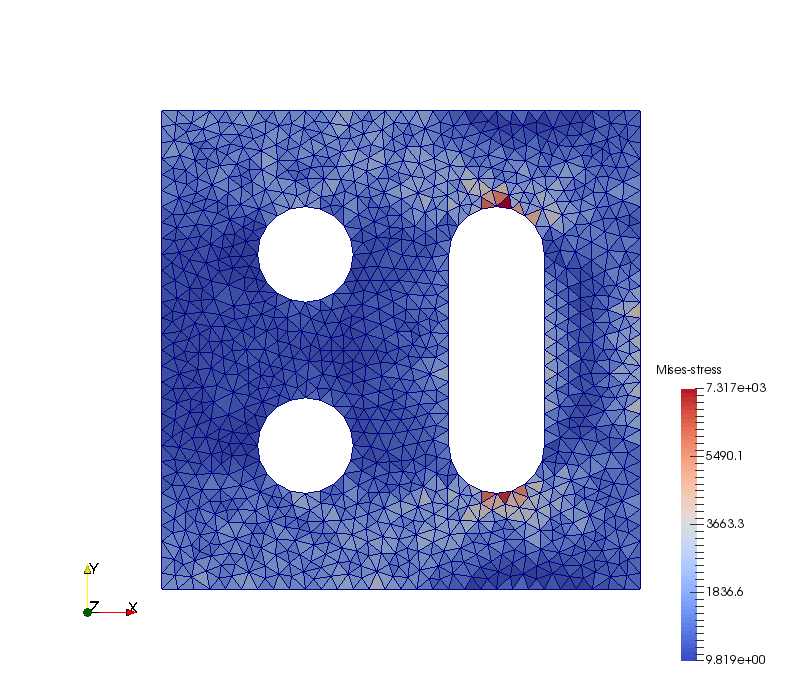
\includegraphics[scale=0.6]{IMG/smile_mises.png}
    \caption{Von Mises stress}
    \label{VonMises}
    \end{center}
\end{figure}